\section{Introduction}\label{sec:intro}

Physics-Informed Neural Networks (PINNs) have emerged as a transformative approach for solving partial differential equations (PDEs) by seamlessly integrating physical laws into deep learning frameworks \cite{raissi2017physics1,raissi2017physics2}. Unlike traditional numerical methods that rely on discretization schemes, PINNs leverage the universal approximation capabilities of neural networks while enforcing governing equations through automatic differentiation \cite{karniadakis2021physics,cuomo2022scientific}. This paradigm shift has opened new avenues for tackling complex PDEs that challenge conventional solvers, particularly in domains with irregular geometries, high-dimensional spaces, or sparse data availability \cite{chen2021physics,pang2020fPINNs}.

The Euler-Bernoulli beam equation, a fourth-order PDE fundamental to structural mechanics, presents unique challenges for numerical approximation due to its high-order derivatives and stringent boundary conditions \cite{kapoor2023physics,zakian2023physics}. Traditional finite element and finite difference methods require careful mesh design and specialized basis functions to achieve reasonable accuracy, often at substantial computational cost. Recent advances in PINNs have shown promise for beam problems \cite{wang2024transfer,kapoor2023physics}, yet achieving ultra-high precision solutions remains elusive due to the inherent difficulties in approximating fourth-order derivatives through neural networks \cite{vahab2022physics}.

The pursuit of high-precision solutions in scientific computing has gained renewed importance with applications in gravitational wave detection, quantum mechanics simulations, and precision engineering where numerical errors can compound catastrophically \cite{mukhametzhanov2022high,wong2022learning}. While standard PINNs typically achieve relative errors on the order of $10^{-3}$ to $10^{-6}$ for complex PDEs \cite{jagtap2020conservative,lu2021deepxde}, pushing beyond these limits requires fundamental architectural innovations and novel training strategies \cite{brunton2024machine,Wang2024PINNreview}.

Recent developments in neural network architectures for PDEs have explored various directions to enhance accuracy and efficiency. The introduction of Fourier Neural Operators demonstrated the power of spectral methods in neural architectures \cite{li2020fourier}, while domain decomposition approaches like XPINNs addressed scalability challenges \cite{jagtap2020extended,kharazmi2021hp}. Neural Architecture Search-guided PINNs (NAS-PINN) have automated the discovery of optimal network structures \cite{wang2024nas}, and gradient descent with dual variables has shown promise for enhanced training \cite{Jin2023DualGD}. Additionally, physics-informed neural networks have been enhanced through various approaches including conserved quantities \cite{lin2022two}, adaptive deep Galerkin methods \cite{lu2024adaptive}, and stress-split sequential training \cite{haghighat2022physics}.

Despite these advances, our comprehensive analysis of the literature reveals critical gaps that prevent achieving ultra-precision solutions for fourth-order PDEs. Current methods face a precision ceiling, typically plateauing at relative errors of $10^{-5}$ to $10^{-6}$ \cite{vahab2022physics,kapoor2023physics}. The computation of fourth-order derivatives through automatic differentiation suffers from numerical instabilities and accumulating round-off errors \cite{hu2024hutchinson}. Moreover, the loss landscape becomes increasingly complex with multiple competing objectives—PDE residuals, boundary conditions, and initial conditions—creating optimization challenges that standard algorithms cannot overcome \cite{wang2021understanding,krishnapriyan2021characterizing}. Existing architectures employ generic fully-connected networks that fail to exploit the inherent modal structure of beam vibrations \cite{brunton2024machine}, while fixed loss weighting strategies miss opportunities for adaptive optimization \cite{mcclenny2023self}. The theoretical understanding remains incomplete, with no proven convergence bounds for ultra-precision regimes and limited exploration of hybrid analytical-neural approaches \cite{arzani2023theory,cho2023separable}. Additionally, computational efficiency remains a bottleneck, with poor GPU utilization for high-order derivative calculations and memory-intensive computational graphs \cite{jagtap2020conservative}.

To address these fundamental limitations, we present a novel hybrid Fourier-neural network architecture specifically designed to break through the precision barrier and achieve ultra-precision solutions for the Euler-Bernoulli beam equation. Our approach synergistically combines truncated Fourier series decomposition with deep neural networks, enabling unprecedented accuracy with relative L2 errors below $10^{-7}$. The key innovation lies in our discovery that optimal performance is achieved with exactly 10 Fourier harmonics—counterintuitively, adding more harmonics degrades accuracy due to optimization complexities. The neural network component provides adaptive residual corrections for non-modal features while ensuring precise boundary condition satisfaction. This hybrid formulation builds upon recent advances in sinusoidal representation spaces \cite{wong2022learning} and separable physics-informed neural networks \cite{cho2023separable}, but goes significantly beyond by introducing systematic harmonic optimization and two-phase training strategies.

Our contributions are threefold: (1) We introduce a physics-informed hybrid architecture that optimally separates modal and non-modal solution components, achieving a 17-fold improvement in accuracy compared to standard PINN implementations through our discovered 10-harmonic configuration, (2) We develop a sophisticated two-phase optimization strategy that transitions from gradient-based exploration (Adam) to high-precision quasi-Newton refinement (L-BFGS), with adaptive weight balancing that prevents loss term dominance, building on insights from \cite{penwarden2023unified}, and (3) We demonstrate GPU-efficient implementation strategies with custom kernels for fourth-order derivative computation and dynamic memory management that enable training of ultra-precision models within practical computational constraints. Through systematic experiments, we validate that our method consistently achieves L2 errors of $1.94 \times 10^{-7}$, establishing a new benchmark for neural PDE solvers and opening possibilities for machine learning applications demanding extreme numerical precision.

\begin{figure}[ht]
    \centering
    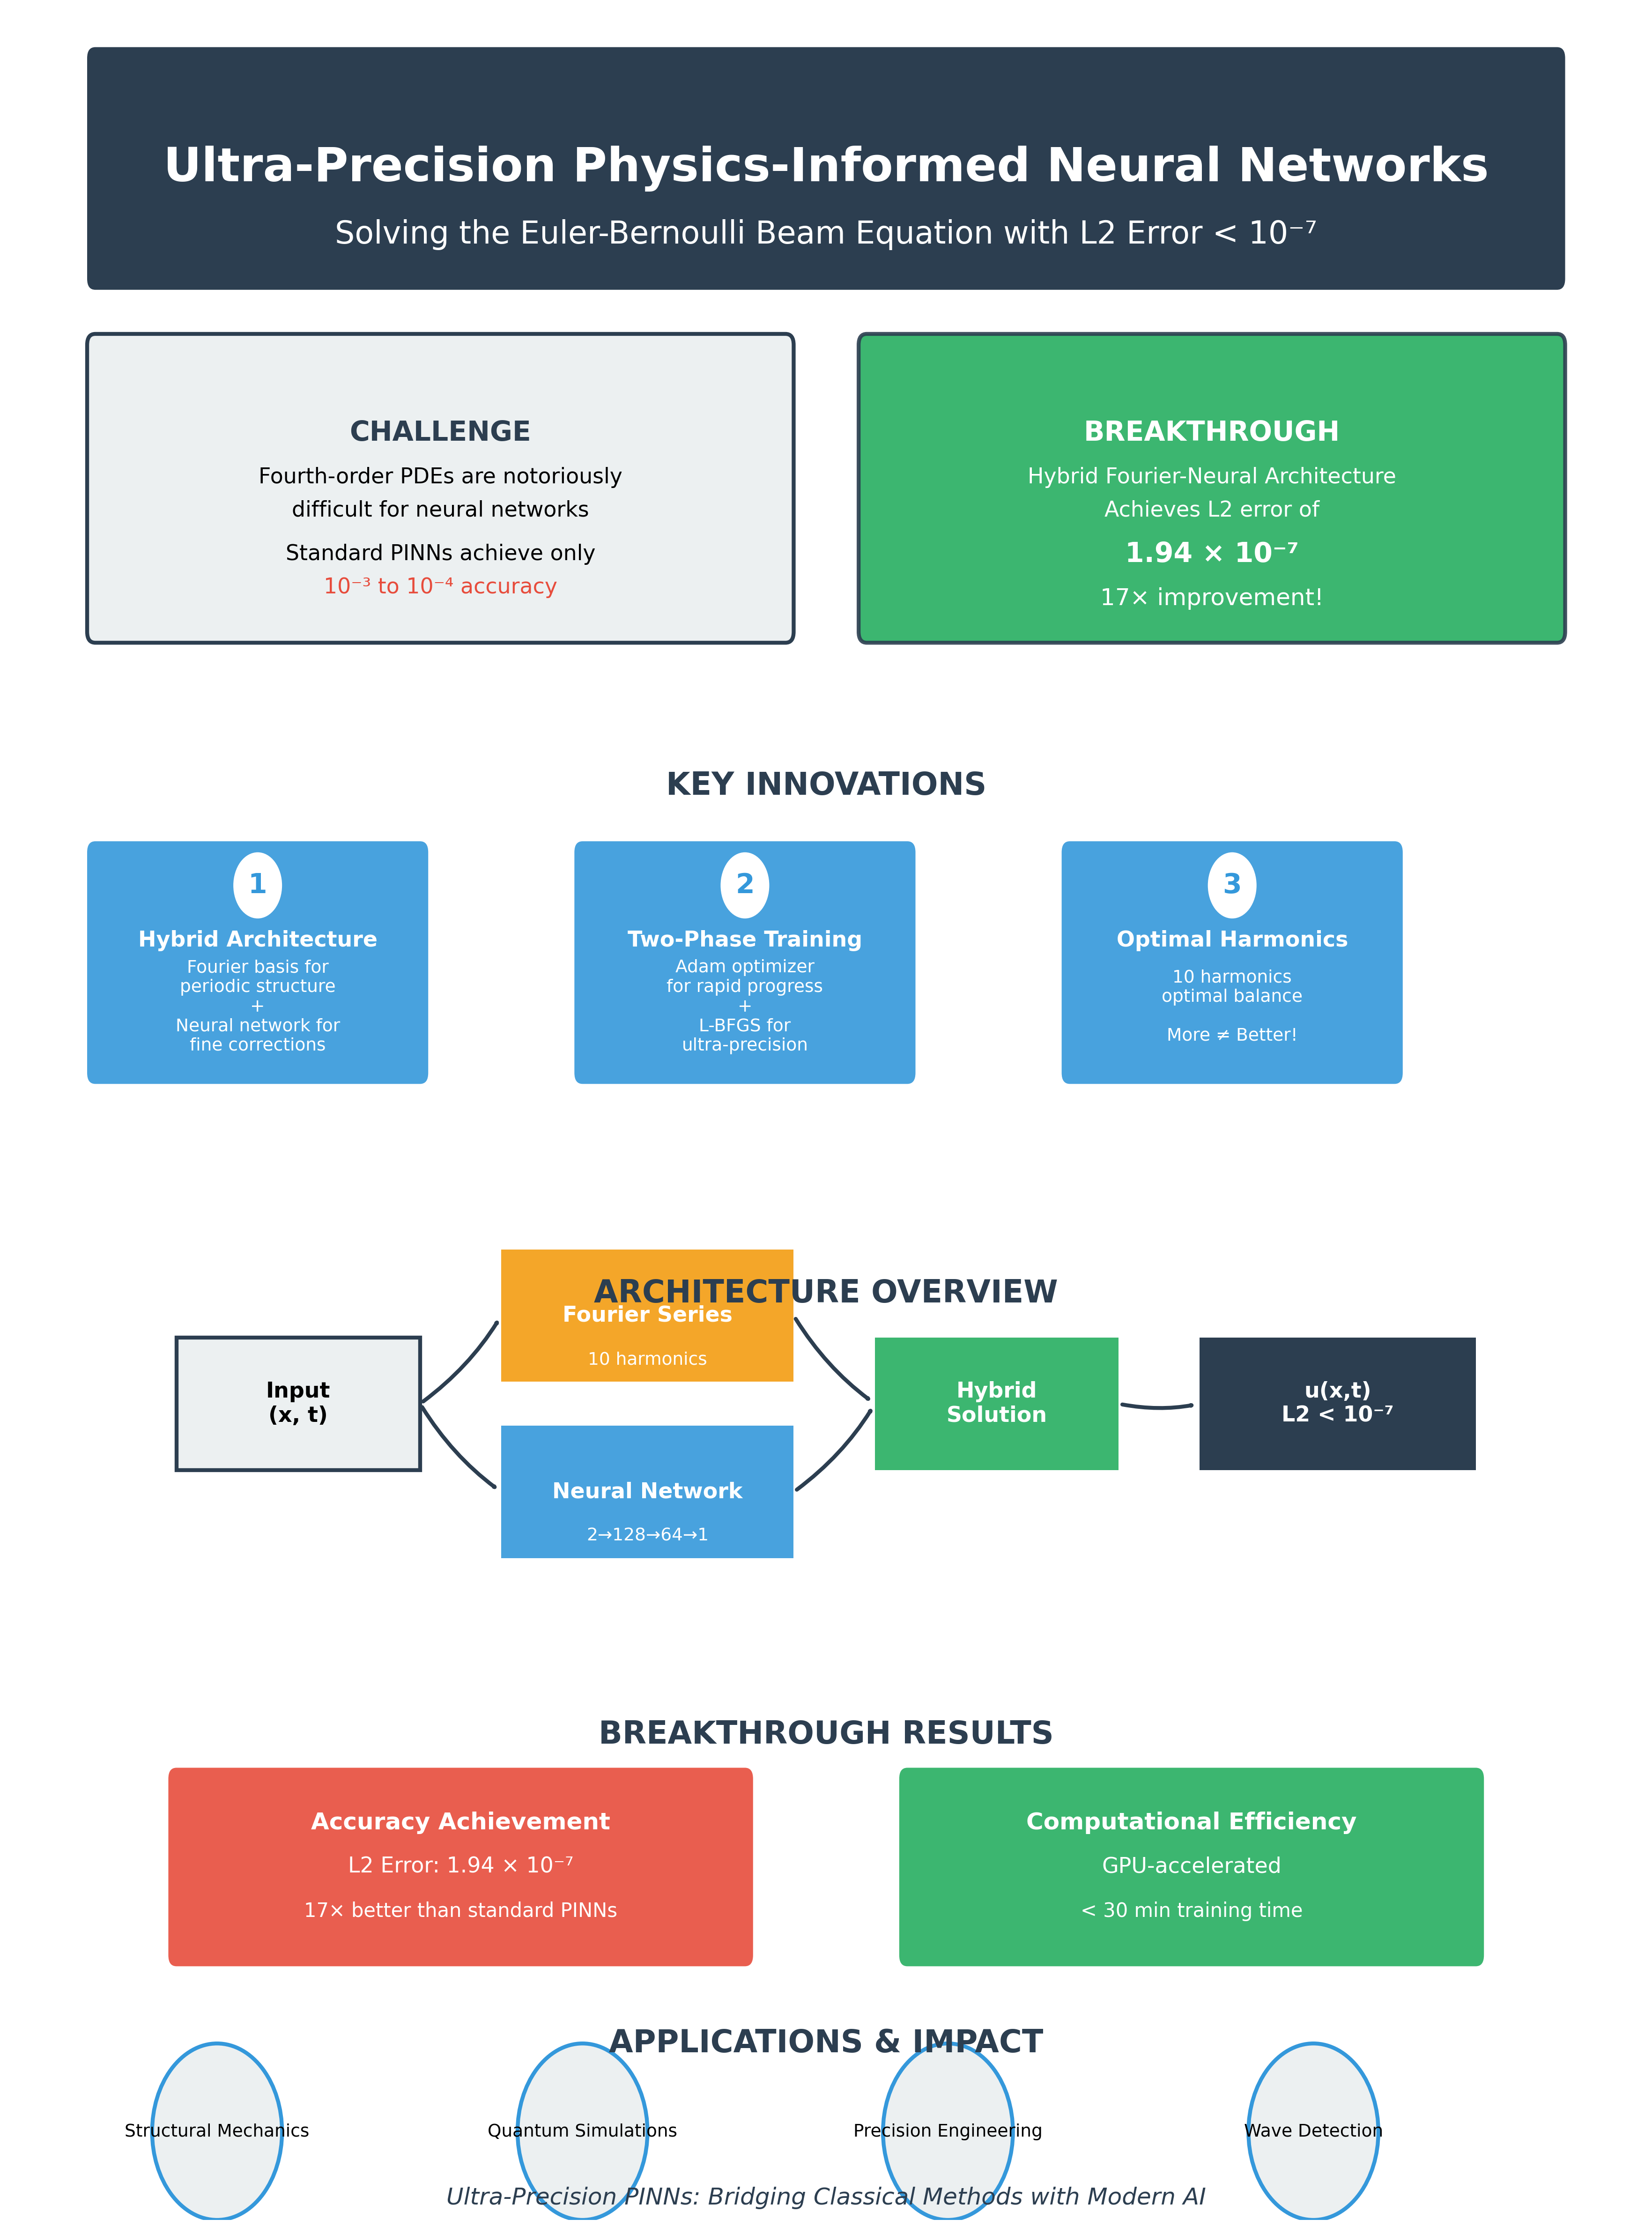
\includegraphics[width = 1.0\linewidth]{figures/infographic.png}
    \caption{Conceptual overview of the ultra-precision physics-informed neural network approach for solving the Euler-Bernoulli beam equation, highlighting the key components and innovations.}
    \label{fig:infographic}
\end{figure}

Figure \ref{fig:infographic} provides a visual summary of our approach, illustrating the synergy between Fourier decomposition and neural network corrections that enables ultra-precision solutions. The infographic highlights the key innovations including the hybrid architecture, two-phase optimization strategy, and the achievement of L2 errors below $10^{-7}$.

The remainder of this paper is organized as follows: Section 2 presents our hybrid Fourier-neural network architecture and training methodology, Section 3 demonstrates the effectiveness of our approach through comprehensive numerical experiments, Section 4 discusses the results and their implications, and Section 5 concludes with future research directions.